\documentclass[a4paper]{article}
\usepackage[utf8]{inputenc}
\usepackage{underscore}
\usepackage[english,serbian]{babel}
\usepackage{graphicx}
\usepackage{color}
\usepackage{url}
\usepackage{float}

\usepackage[unicode]{hyperref}
\hypersetup{colorlinks, citecolor=green, filecolor=green, linkcolor=blue, urlcolor=blue}

\begin{document}

\title{Nanotehnologija i primene\vspace{0ex}\\
\small{Seminarski rad u okviru kursa\\
Tehničko i naučno pisanje\\
Matematički fakultet}\vspace{3ex}}
\author{
Petar Đerić\\
mi20135@alas.matf.bg.ac.rs\\\\
Ivan Tešović\\
mi20111@alas.matf.bg.ac.rs\and
Luka Mijailović\\
mi22100@alas.matf.bg.ac.rs\\\\
Uroš Cvetković\\
mi22065@alas.matf.bg.ac.rs
}
\date{13. Novembar 2022.}

\maketitle

\abstract{U narednom tekstu ćemo se ukratko upoznati sa pojmom \textbf{nanotehnologije.} Na početku ćemo govoriti o istoriji (razvoju nanotehnologije), nakon čega će biti reči o \textbf{nanomaterijalima}, kao i o njenim \textbf{primenama} u raznim interesantnim oblastima.
 
\tableofcontents                 
\newpage

\section{Uvod}
\label{sec:uvod}
\sloppy \textbf{Nano} predstavlja milijarditi deo metra i bez mikroskopa uopšte nije vidljiv. Materijali se u sitnijoj razmeri ponašaju sasvim drugačije nego u većem obliku. Da bi se omogućilo poboljšanje performansi i osobina materijala, \textbf{nano čestice} su u sve većem fokusu istraživanja.\\ Osnovni cilj izučavanja na ovom nivou jeste sposobnost razumevanja materijala na \textbf{nano-lestvici}. Ove mikro veličine su bitne kada se proučava susret dva materijala.\\ Kod dimenzija u opsegu do 100 nm, pojave kvantne fizike preovladavaju nad pojavama klasične fizike. Bitna je činjenica da manja tela imaju znatno veći odnos broja atoma na površini i broja atoma u unutrašnjosti od većih tela.\\ Ti odnosi na mikro nivou dovode do razumevanja kompletne strukture materijala, a mogućnost upravljanja složenim strukturama se vrši upravo u nano području. Nevidljiva revolucija ima tendenciju da preraste u novu industrijsku revoluciju.


\section{Nanotehnologija}

\subsection{Nastanak i razvoj nanotehnologije}
\sloppy Iako se nanotehnologija smatra modernom naukom, njeni počeci se vezuju za duboku prošlost.
Termin \textit{nanotehnologija}, prvi je upotrebio \textbf{Norio Taniguči} (Slika \ref{slika_Norio}) sa Univeziteta u Tokiju 1974. godine govoreći o proizvodnji materijala u slučaju kada je tolerancija na grešku reda \textbf{nanometra}.
Krajem 1980-ih, pojam nanotehnologija ulazi u široku upotrebu za opis budućih tehnologija koje će se bazirati na molekularnim mašinskim sistemima koji su dizajnirani tako da budu sposobni za konstruisanje složenih proizvoda sa atomskom preciznošću.\\ 
Od sredine 1990-ih, upotreba koncepta se proširila na instrumente, procese i proizvode čije su ključne dimenzije u rangu između 1 i 100 nanometara.\\

\begin{figure}[H]
    \centering
    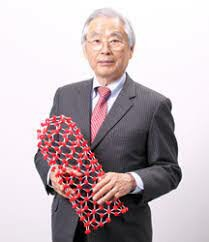
\includegraphics[width=.4\textwidth]{slika 1.jpg}
    \caption{Norio Taniguči}
    \label{slika_Norio}
\end{figure}

\subsection{Pojam nanotehnologije}
\textbf{Nanotehnologija} \cite{prviLink} je interdisciplinarna nauka koja uključuje fiziku, hemiju, biologiju, nauke o materijalima, kao i širok skup inženjerskih disciplina.\\ 
Danas, nanotehnologija kao inženjerska disciplina, odnosi se na tehnike i proizvode koji uključuju strukture nanometarskih dimenzija ( od 1 do 100 nanometara).\\  Reč \textit{nanotehnologija}, koristi se kao sinonim i za \textbf{nauku} i za \textbf{tehnologiju}.\\ 
Kao nauka, nanotehnologija proučava fizičke, hemijske i biološke osobine molekula i atomskih čestica. Kao tehnologija, primenjuje istraživanja iz navedenih nauka i različite inženjerske discipline za proizvodnju materijala i funkcionalnih sistema sa posebnim osobinama.

\subsection{Ciljevi i mogućnosti nanotehnologije}
Progres u nanotehnologiji se može posmatrati preko mnogih parametara, uključujući preciznost, složenost, isplativost i izbor proizvoda.\\ 
Dugoročni ciljevi nanotehnologije su atomska preciznost, ušteda u proizvodnji, kao i masovna proizvodnja. Kombinacija ovih ciljeva deluje izvodljivo, ali samo kroz višeslojni proces koji počinje sa razumjevanjem da je trenutno stanje razvoja nanotehnologije ograničenih sposobnosti.

Tehnologije koje se koriste u nanotehnologiji su veoma različite, brzo se menjaju i često nisu međusobno povezane. Tipični proizvodi nanotehnologije su \textbf{nanočestice}, \textbf{fibre} i \textbf{filmovi} različitih materijala i struktura. 
Mediji i materijali koji se koriste za proizvodnju nanostruktura i nanotekstura nalaze praktičnu primjenu počev od proizvodnje odeće otporne na fleke, pa sve do naprednih elektronskih komponenti.

Sa razvojem nanotehnologije, razviće se nove metode lečenja koje su bazirane na upotrebi nano-robota, popularno nazvanih nanobotovi (eng. nanobots). Već su razvijeni materijali koji se mogu samopopravljati (eng. self-healing materials) i to je verovatno pravac kojim će se oblast proizvodnje novih materijala kretati.\\
Budućnost bi trebalo da donese razvoj aktivnih nanostruktura, zatim konkretnih funkcionalnih nanosistema, i konačno polovinom ovog veka i do razvoja savršenih molekularnih nanosistema.

\section{Nanomaterijali}

\sloppy Nanotehnologija je omogućila stvaranje materijala koji uključuju nanooblike, što je veoma korisno jer oni imaju mnoge prednosti. \textbf{Nanomaterijalima} \cite{drugiLink} se smatraju objekti kojima je bar jedna dimenzija između 1 i 1000 nanometara, što je uobičajena definicija nanoskale. Ono što nanomaterijale čini posebnim je da se njihove fizičke i hemijske osobine mogu razlikovati od materijala iste vrste koji imaju makroskopske dimenzije. Jednostavno govoreći, ovi objekti se ponašaju drugačije samo zato što su mali. Jedan od najvećih izazova sa kojima se nanotehnologije suočavaju je kontrolisana manipulacija nano-objektima. Nanomaterijali bazirani na ugljeniku su verovatno najviše ispitivani sistemi. Sintetisani su kao 1D (\textbf{ugljenične nanocevi}), 2D (\textbf{grafen, grafen-oksid}), i 3D (\textbf{fulereni}) nanostrukture.\\
Najzastupljenije su \textbf{nanocevi} (Slika \ref{slika_nanocevi}) koje mogu biti \emph{jednoslojne} i \emph{višeslojne}. 

\begin{figure}[H]
    \centering
    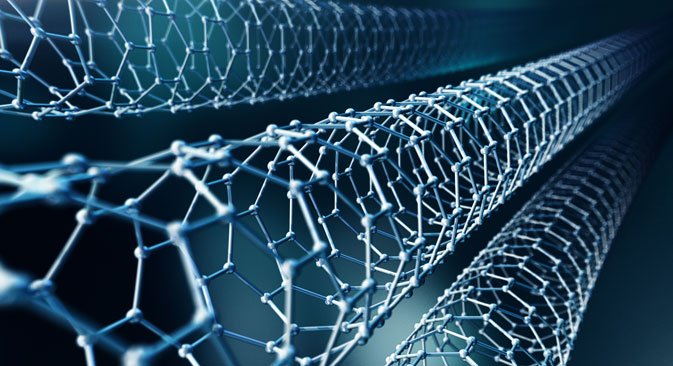
\includegraphics[width=.6\textwidth]{slika 2.jpg}
    \caption{Ugljenične nanocevi}
    \label{slika_nanocevi}
\end{figure}

Najčešća upotreba nanocevi je za proizvodnju kompozitnih materijala.\\

\textbf{Grafen}, najtanji materijal ikada napravljen, koristi se u elektronici, farmaciji i medicini. Zbog svoje specifične površine idealan je kao nosač za druge nanostrukture.\\

Otkriće grafena uticalo je na razvoj čitave klase \textbf{2D nanomaterijala}. Ovi materijali imaju lisnatu strukturu (nano-listići) i pokazuju jako interesantne elektronske osobine i tvrdoću. Oni imaju veliku primenu u elektronici i optoelektronici. Pokazano je da se mogu koristiti za proizvodnju tranzistora sa pojačanim efektima električnog polja i kao fotodetektori.\\

\textbf{Fuleren} (Slika \ref{slika_fuleren}) je laserski sintetizovan još 1985. godine. Sastoji se od 60 hibridizovanih ugljenikovih atoma. Fulereni su najkorišćenije nanočestice posle srebra.\\ 

\textbf{Kvantne tačke} su nanočestice koje imaju prečnik od nekoliko nanometara i mogu se podešavati tako da emituju svetlost određene boje. Ova činjenica ih može učiniti korisnim za \emph{detekciju}. Pri osvetljavanju belom bojom svaka nanočestica će emitovati svetlost jedne boje, čiji je intenzitet i do hiljadu puta veći od trenutno korišćenih testova.\\

\textbf{Nanoljuske} se sferne nanočestice. Sastoje se od \emph{jezgra} i tanke \emph{zlatne ljuske}. Ove nanočestice se najviše koriste za \emph{uništavanje ćelija tumora}. Nanoljuske kruže po organizmu dok se ne akumuliraju blizu ćelija tumora. Na željenom mestu nanoljuske apsorbuju infracrvene talase što izaziva otpuštanje leka u lokalizovanoj zoni.\\


\begin{figure}[H]
    \centering
    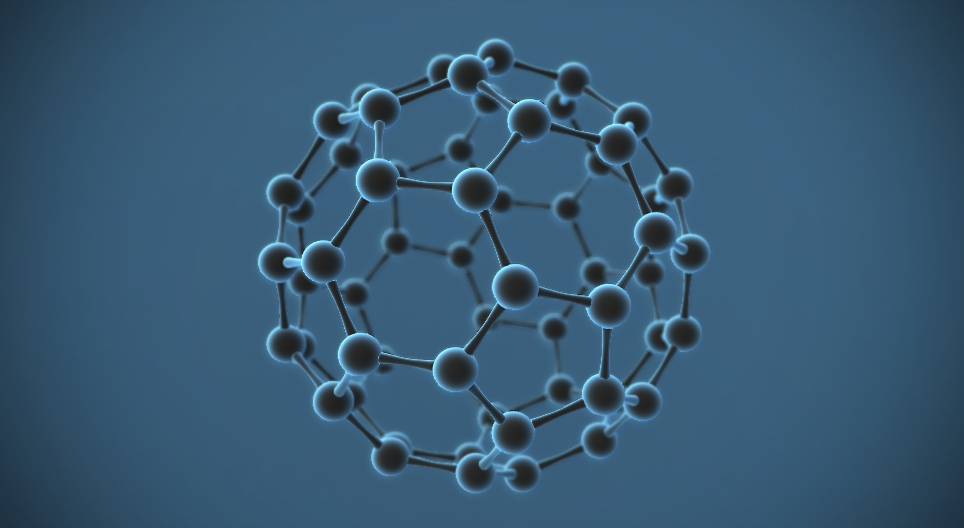
\includegraphics[width=.4\textwidth]{slika 3.jpg}
    \caption{Struktura fulerena}
    \label{slika_fuleren}
\end{figure}

\section{Primena nanotehnologije}
\textbf{Nanotehnologija} ima široku primenu \cite{treciLink}: 
\begin{itemize}
    \item[1] IT industrija
    \item[2] Automobilska industrija
    \item[3] Medicinska industrija 
    \item[4] Kvantna mehanika
    \item[5] Robotika
\end{itemize}

Pošto su primene nanotehnologije velike, mi ćemo vam predstaviti primenu u IT industriji i u automobilskoj industriji.\\


\subsection{IT industrija}

\textbf{IT industrija} je doživela veliku revoluciju zahvaljujući nanotehnologiji. Veliki napredak je postignut u računarstvu i elektronici, što je dovelo do bržih i manjih sistema koji mogu da upravljaju sve većim količinama informacija.\\
\subsubsection{Tranzistori}
\textbf{Tranzistori} \cite{cetvrtiLink}, osnovni prekidači u modernim računarima, postali su sve manji kroz nanotehnologiju. Nekada tipičan tranzistor je bio veličine 130 do 250 nanometara. Intel je 2014. godine napravio tranzistor od 14 nanometara, zatim je IBM 2015. napravio prvi tranzistor od samo 7 nanometara. (Slika \ref{slika_4}) Manji, brži i bolji tranzistori mogu značiti da će uskoro cela memorija vašeg računara biti uskladištena na jednom malom čipu.\\

\begin{figure}[H]
    \centering
    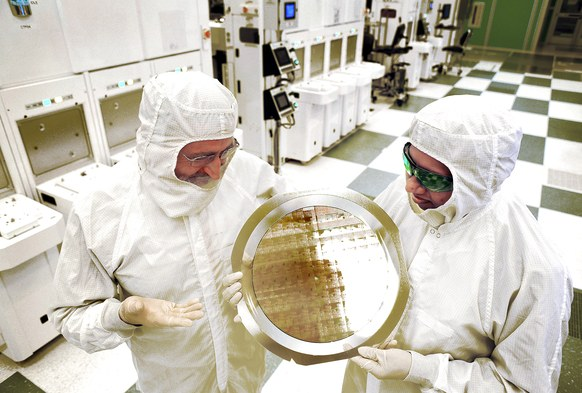
\includegraphics[width=.6\textwidth]{slika 4.jpg}
    \caption{IBM pločice čipova od 7nm}
    \label{slika_4}
\end{figure}

Sada se prodaju \textbf{ekrani} i \textbf{televizori} ultra visoke definicije koje korsite kvantne tačke za proizvodnju živopisnijih boja, a istovremeno su energetski mnogo efikasniji.\\

\subsubsection{Elektronika}
Fleksibilna, sklopiva, savitljiva i rastegljiva, \textbf{elektronika} doseže u različite sektore i integriše se u različite proizvode, uključujući nosive uređaje, medicinske aplikacije, aplikacije u vazduhoplovstvu i Internet stvari. Fleksibilna elektronika je razvijena korišćenjem, na primer, poluprovodničkih nanomembrana za aplikacije u ekranima pametnih telefona i e-čitača. Drugi nanomaterijali kao što su grafen i celulozni nanomaterijali se koriste za različite vrste fleksibilne elektronike kako bi se omogućili nosivi i  fotonaponski uređaji koji se mogu zašiti na odeću i elektronski papir koji se može umotati. Pravljenje ravne, fleksibilne, lagane, nelomljive, visoko efikasne elektronike otvara vrata za bezbroj pametnih proizvoda u IT industriji.

\section{Primena nanotehnologije u automobilskoj industriji}

\begin{table}[h!]
\begin{center}
\begin{tabular}{|c|c|}
\hline
Deo automobila & Nanomaterijal koji se koristi \\
\hline
Spoljašnjost & nano-lak \\
\hline
Karoserija & nanočelik \\
\hline
Unutrašnjost & nano filter \\
\hline
Šasija i gume & crni ugljenik \\
\hline
\end{tabular}
\end{center}
\end{table}

\subsection{Primena nanotehnologije u proizvodnji karoserije automobila}

U domenu površinskih tehnologija, nanostrukturisane površine mogu poboljšati, npr. prijanjanje boje na površinu. Otpornost na grebanje i prljavštinu pa samoobnovljiva boja već postoji ili je u razvoju. Osim boje, nanotehnologija razvija ultra tanke premaze za stakla, ogledala i reflektore na karoseriji automobila.\\

\textbf{Nano-lak} kojim se premazuju automobili daje automobilu veću otpornost na ogrebotine i bolji sjaj u odnosu na konvencionalne boje. Konvencionalne boje se sastoje od veziva i unakrsno povezanih stvari, a nanoboje se sastoje od organskih veziva sa velikom elastičnošću i neorganskih nanočestica s velikom čvrstoćom (Slika \ref{slika_6}). Korištenjem nano-laka sjaj se neće izgubiti nakon brojnih pranja automobila.\\

Bazu navedenog efekta (nano-laka) predstavljaju ugrađene keramičke čestice u završnom sloju laka. Baza je nanostrukturirani prah proizveden u gasovitom stanju sinteze u plamenu (veličine 7 do 40 nm). 
Ako je rastvor boje tečnost, navedeni delovi su inicijalno nasumično raspoređeni u navedenom rastvoru. Tokom sušenja i procesa paljenja oni se mešaju s molekularnom strukturom boje što rezultira gustom i uređenom matricom na površini boje. Tako je otpornost na ogrebotine tri puta poboljšana te se sjaj boje znatno popravio. Ovaj novi način bojenja automobila je razvijen od kompanije „\textit{Daimler-Chrysler}“-a, a koriste ga već neki modeli „\textit{Mercedes-Benz}“-a. \\

Procedura za kaljenje nanoboja koja podnosi visoke temperature je bazirana na korištenju specijalnih infracrvenih reflektora. Takve reflektore proizvodi kompanija „\textit{Heareus}“ smeštena u Hanau.

\begin{figure}[H]
    \centering
    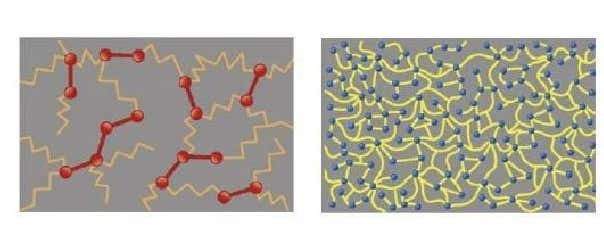
\includegraphics[width=.7\textwidth]{slika 6.jpg}
    \caption{Poređenje konvencionalne boje (levo) i boje sa nanočesticama (desno)}
    \label{slika_6}
\end{figure}

Danas se koristi oko 6 $m^{2}$ stakla kod proizvodnje automobila – \\1.2 $m^{2}$ samo za zaštitu od vetra. Zaključujemo potrebu za laganim staklima što se postiže zamenom mineralnih stakala polimerskim staklom. Mora biti otporan na ogrebotine, abraziju i klimatske promene. \\

Polimerska stakla, posebno polikarbonat s odličnim svojstvima (velika čvrstoća i mala težina), se već serijski koriste pri izradi prednjih svetala i sočiva. \\

Nove mogućnosti donosi čvrsta plastika otporna na ogrebotine. Budući da se plastika lako formira donosi nove mogućnosti u dizajnu – od krovova automobila i tela automobila do celih modela automobila napravljenih od plastike s integrisanim svetlima i aerodinamičnim elementima (Slika \ref{slika_7}).

\begin{figure}[H]
    \centering
    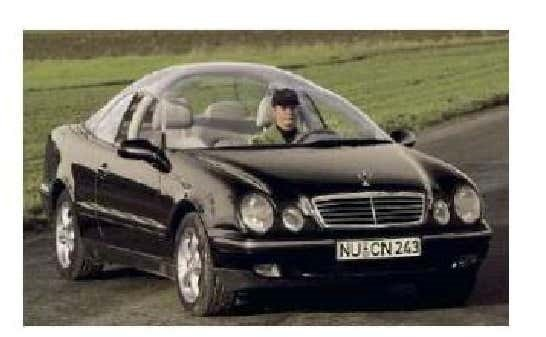
\includegraphics[width=.5\textwidth]{slika 7.jpg}
    \caption{Testni automobil sa staklenim krovom}
    \label{slika_7}
\end{figure}

\newpage

\section{Zaključak}
Moderna nauka oslanja se na razvoj nanotehnologija, koje se danas primenjuju u svim sferama naučnih istraživanja – u \textbf{industriji}, \textbf{medicini}, \textbf{kozmetici}, pa i u svakodnevnom životu. Tehnologija je veoma uticala na tok istorije i prirodu ljudskog društva, i to nastavlja i danas, a tako će biti i u budućnosti. Po rečima i očekivanjima mnogih nanotehnologija će obeležiti dvadeset prvi vek i ustoličiće se kao imperativ stalnog razvoja. Istaknuti naučnici smatraju da je nanotehnologija pravi odgovor na ključne probleme današnjice koji ujedno određuju svetlu budućnost čovečanstva. Ova tehnologija razvija se u poslednjim decenijama neverovatnom brzinom, ali još uvek je u ranoj fazi komercijalizacije. Ono što je takođe vrlo važan zadatak je da \textit{nanomašine} i uređaji treba da budu komplementarni i kompatibilni sa biološkim sistemima, u prvom redu sa čovekom. Prednosti koje ova nova tehnološka ideja nosi sa sobom mnogobrojne su i veoma značajne za razvoj čovečanstva, ali donose i upozorenja, strahove i pozivaju na oprez. Gledano sa tog aspekta nanotehnologija može obezbediti da čovek postane „\textbf{kosmičko biće}“ tj. da bezbedno putuje kosmičkim prostranstvima. Velika moć koju sadrži novi tehnološki pogled na svet ima visoku cenu, a koliko visoku, pokazaće decenije pred nama. Svakog dana se pojavljuje neka nova ideja o upotrebi nanotehnologije i veoma je zanimljivo pratiti šta univerziteti, velike IT kompanije, medicinski i hemijski
instituti i drugi imaju da podele sa javnošću. Baš zbog toga mnogi kažu da je nanotehnologija sledeća \textbf{tehnološka revolucija}. Zato je potrebno da obrazovni sistemi u svim zemljama sveta prate razvoj novih tehnologija i prilagode se promenama. U suprotnom neće nam biti jasno šta ćemo raditi u budućnosti, jer za nove poslove treba novo znanje.

\newpage

\begin{thebibliography}{9}
\bibitem{prviLink} \url{https://www.industrija.rs/vesti/clanak/nanotehnologije-istorijat-sadasnjost-i-pogled-u-buducnost}
\bibitem{drugiLink} \url{https://www.mdpi.com/journal/nanomaterials}
\bibitem{treciLink} \url{https://www.nano.gov/about-nanotechnology/applications-nanotechnology}
\bibitem{cetvrtiLink} \url{https://scitechdaily.com/nanotechnology-advance-enables-tinier-transistors-with-extraordinary-performance/}
\bibitem{petiLink} \url{https://www.azonano.com/article.aspx?ArticleID=4936}
\end{thebibliography}

\end{document}
